\chapter{Introduzione}
    L'oggetto della tesi \'e una relazione dettagliata sul progetto di stage universitario svolto presso DDX,
    una software house che si occupa dello sviluppo di software CAD/CAM
    \footnote{\textbf{Software CAD/CAM} - Un software CAD/CAM è un programma che consente la progettazione (CAD)
    e la realizzazione (CAM) di manufatti in diversi materiali, come il legno, il vetro o la pietra, tramite 
    l'uso di macchine a controllo numerico (CNC).}.\\

    \begin{figure}[h]
        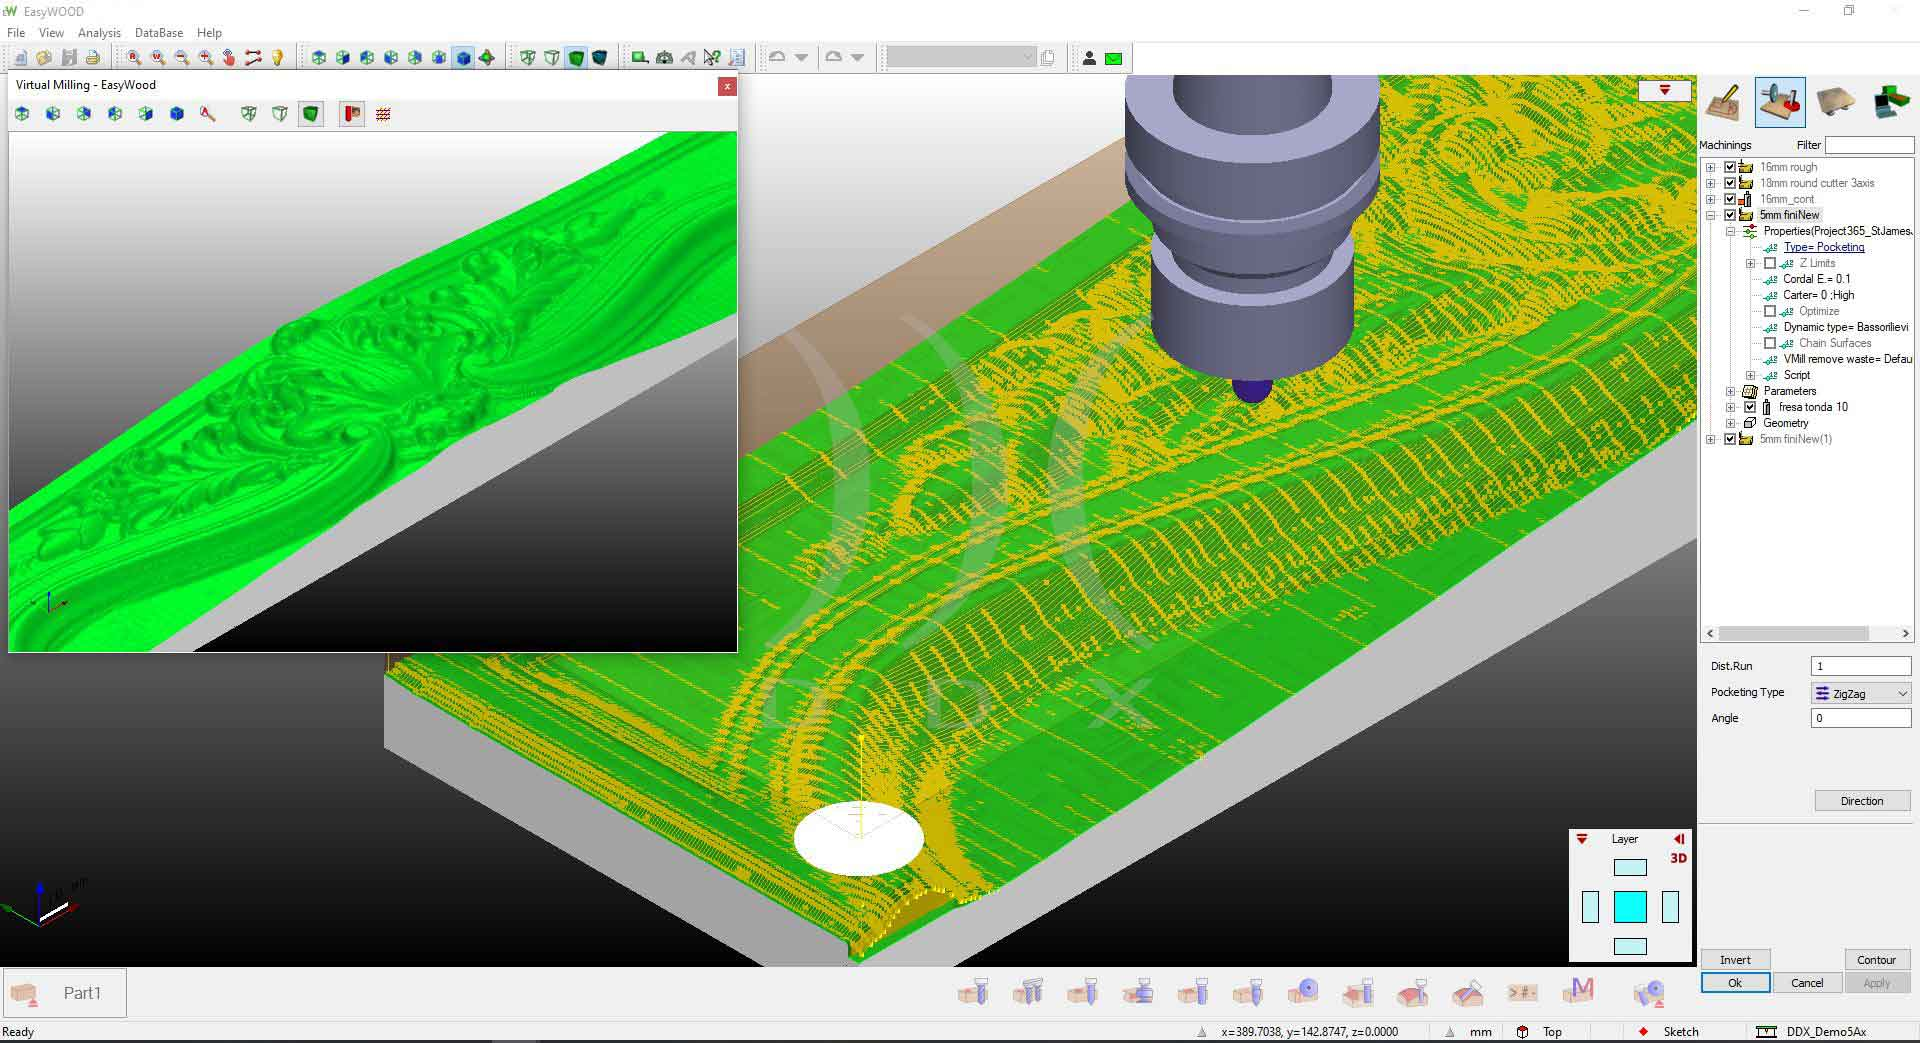
\includegraphics[width=\textwidth]{images/easywood.jpg}
        \caption{Uno dei Software di CAD/CAM sviluppato internamete}
    \end{figure}

    Il risultato questo periodo di sviluppo, durato in totale 3 mesi, \'e un report web dinamico per la consultazione e la modifica dei test. 
    In questa tesi verranno discusse le tecnologie, le scelte tecniche e la struttura dell'applicazione.\\

    Per essere meglio compreso il funzionamento dell'applicativo verr\'a illustrata nello specifico la struttura del sistema di test.\\
    Successivamente verr\'a descritta una panoramica del flusso di sviluppo e come il report in oggetto si integri con esso. \\
